
%use mybib.bib for bibliography. bibtex is used for bibliography
\documentclass[journal]{IEEEtran}
\usepackage[utf8]{inputenc}
\usepackage{graphicx}
\usepackage{cite}
\usepackage{longtable}
\usepackage{amsmath}
\usepackage{multirow}
\usepackage{multicol}
%\usepackage{wrapfig}
\usepackage{float}
%\usepackage[section]{placeins}
%\usepackage{subcaption}
\usepackage{array}
\usepackage[export]{adjustbox}
\usepackage{tabu}
\usepackage{listings}
\usepackage{siunitx}
\usepackage{siunitx}



%%%%%%%%%%%%%%%%%%%%%%%%%%%%%%%%%%%%%%%%%%%%%%%%%%%%%


\ifCLASSINFOpdf

\else

\fi


\hyphenation{op-tical net-works semi-conduc-tor}


\begin{document}

\title{A* Based Optimum Control of Enterprise Level Energy Storage Based on Forecasting of PV, Load and Real-Time price of Energy}

\author{Alvi Newaz, Juan Ospina, Omar Faruque}






\maketitle                                                               

\begin{abstract}
Optimizing energy storage management based on present and forecasted data is necessary for efficient operation of distributed energy resources. The purpose of this paper is to present a technique based on A* search algorithm \cite{a8book} to optimize the use of energy storage. The energy management problem is represented as a graph and A* search algorithm is used to find the optimum actions from the graph to get the minimum cost of operation. A case study has been done using the feeder 2 from the SUNGRIN project \cite{SUNGRIN} and the results are presented.


\end{abstract}



\IEEEpeerreviewmaketitle



\section{Introduction}
In the last few years, there has been significant growth in grid-connected distributed energy resources (DERs) leading to an increased deployment of distributed generation (DG) and recently more distributed storage (DS) systems. Companies are starting to heavily invest in the competitive energy storage system market by taking advantage of the decreasing costs of energy storage. Although a significant amount of DG and DS are being added to the distribution grid, need to improve their control systems for seamless integration to the grid is still there. In the US, most DG and DS systems are deployed to either help reduce the metered load through net-metering programs or to sell power to the utility through power purchase agreements (PPAs). The potential of DG combined with DS is not fully utilized under these pricing schemes due to the lack of proper control. in order to maximize the use of available DERs, a state-of-the-art energy management solution is a necessity for our future electrical grid . Such an energy management solution will be able to dynamically optimize the use of all the available DS with the objective of serving the load in the most economical and safe way possible. This will benefit both utility companies and regular consumers. Due to the constraints and intermittent nature of some DG systems, such as wind and solar, the optimum management of DS combined with a DG is a difficult problem to solve. The most common approaches found in the current literature are as follows. Some researchers formulate the problem as a linear programming (LP) or mixed integer linear programming (MILP) model \cite{lp73, lp74, lp75}. Authors in \cite{pso80, pso81} present an energy management solution based on particle swarm optimization for a microgrid containing wind turbines and energy storage (ES) system. Other researchers propose crow-search and ant colony optimization models to solve the energy management problem for local microgrids as seen in \cite{csa87} and \cite{aco84}. There have also been model predictive control (MPC) based approaches for managing ES in microgrid settings as seen in \cite{energymanajaboulay,mpcmorstyn}.  Researchers in \cite{ga76, ga77} have also proposed genetic algorithm based solutions to optimize the ES operation in a microgrid. One clear disadvantage of these proposed models is that most of these approaches only consider the current status of the system and ignore some critical factors like energy tariff, forecasted load, and forecasted generation profiles.  These information can be used to find an optimum solution based on both current and probable future states of the system as opposed to a solution relying only on the currently available data. Off-line day ahead planning models have also been proposed in the literature. In these methods, available predicted data is used to optimize the scheduling of the ES based on Monte Carlo simulations \cite{6872821,7010943,6839110}. These solutions are very computationally intensive and require a lot of time for planning the day ahead. The computational complexity makes them unsuitable for real-time implementation. Also, as they are off-line calculations they rely vastly on the accuracy of the predictions.

From the discussion thus far, it is evident that there is a need for a real-time ESM solution that can optimize the long-term operating costs of a system containing DG and an energy storage (ES) system. This paper presents an optimum real-time control strategy for such systems. The proposed control strategy takes into account the present and forecasted states of the system, together with the real-time price (RTP), in order to optimize the cost of energy usage. The rest of the paper is organized as follows. Section II discusses how the ESM problem is formulated as a graph search problem. Section III introduces the A* graph search algorithm used to find the optimal solution and how it is used to search for the optimum path of energy decisions. Section IV discusses the test system used in simulation to validate the performance of the graph search based ESM algorithm. Section V discusses the results obtained from the offline simulation and section VI presents the real-time simulation results. Section VII talks about the novelty of the research and section VIII presents the conclusions.

\section{Problem formulation}
The proposed solution technique is designed to be implemented at the point of common coupling (PCC) of a microgrid containing distributed generation (DG) and energy storage (ES). Fig. \ref{fig:system_arch} depicts an example system. Here, the energy storage management system (ESMS) is in charge of controlling the battery connected to the grid with the objective of getting the most cost optimum use of the resources available. The objective of the ESMS is to optimize the use cost of energy storage under different pricing schemes by taking advantage of RTP or time of use (TOU) prices, load and DG generation forecasting.  Fig. \ref{fig:F1_CA} shows the top-level architecture of the ESMS. As seen in the figure, the inputs of the system are the real-time price (RTP) prediction, load prediction, and the DG output prediction, which in this case is a photovoltaic (PV) plant output. It will also consider the current state of the load, current PV generation, and the state of charge of the ES. The output of the ESMS is the optimum battery charge and discharge control references based on the current and forecasted data.

\begin{figure}[!htbp]
\centering
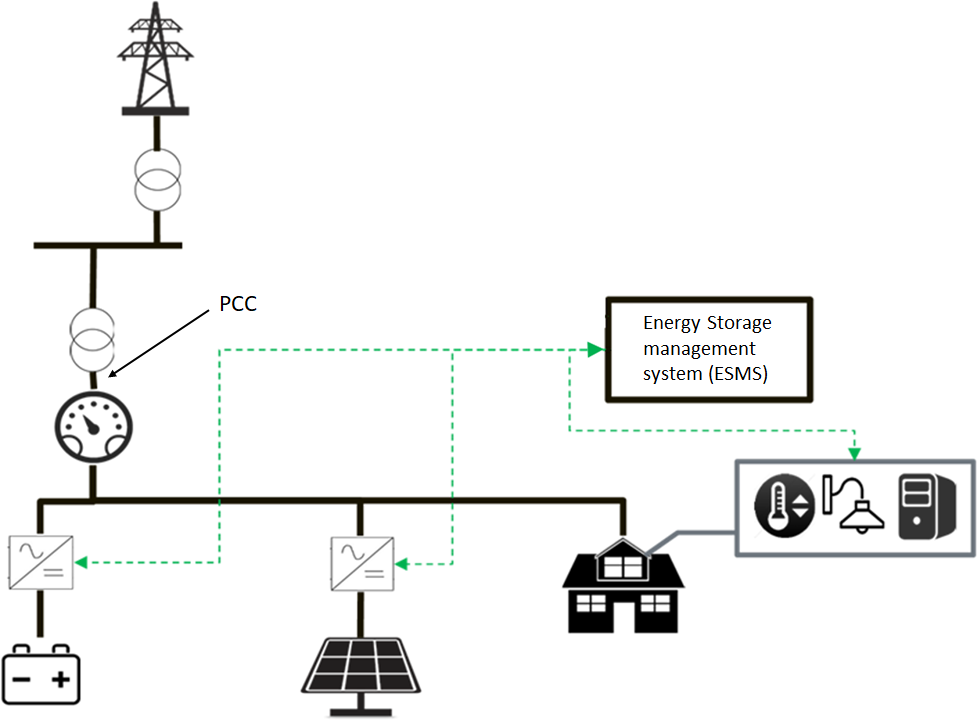
\includegraphics[width=\linewidth]{figs/System_architecture.png}
\caption{Test system architecture}
\label{fig:system_arch}
\vspace{-3mm}
\end{figure}

%  Fig. \ref{fig:F1_CA} shows the top-level architecture of the ESMS. As seen in the figure, the inputs of the system are the real-time price (RTP) prediction, load prediction, and the DG prediction, which in this case is a photovoltaic (PV) plant. It will also consider the current state of the load, PV generation, and ES. The output of the ESMS is the optimum battery charge and discharge control references based on the current and forecasted data.

\begin{figure}[!ht]
    \centering
    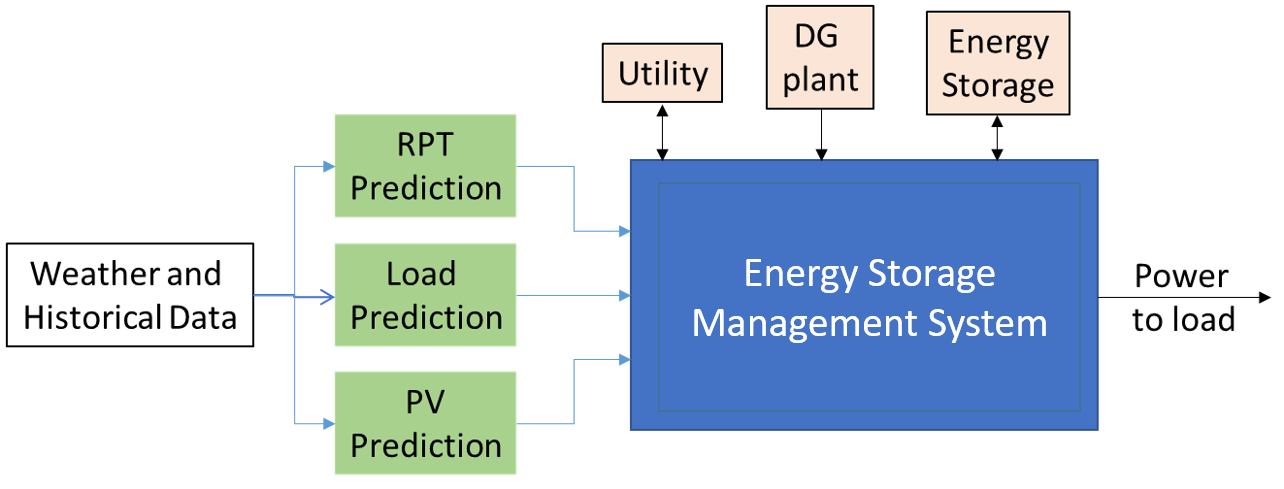
\includegraphics[width = \linewidth]{figs/EMS_FIG.png}
    \caption{Controller top level architecture}
    \label{fig:F1_CA}
\end{figure}

In order to find the optimum cost solution based on the current status of the system and future forecasts, the optimization problem is formulated using a graph search problem approach. To represent the solution space of the problem as a graph, the state of charge (SOC) of the ES, and both the prediction horizon and the control horizon are discretized. Fig. \ref{fig:F1_Dis} demonstrates an example of the discretized solution space.
\begin{figure}[!ht]
    \centering
    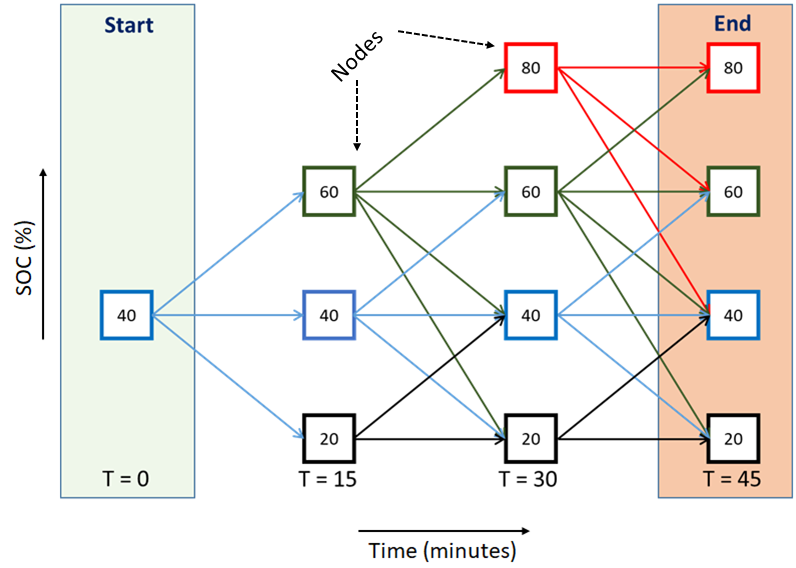
\includegraphics[width = \linewidth]{figs/F1_1_Dis.png}
    \caption{Discretizing solution space}
    \label{fig:F1_Dis}
\end{figure}
The horizontal axis of the figure represents time, and the vertical axis represents discrete steps in the state of charge (SOC) of the energy storage. In this simple example scenario, it is assumed that the algorithm recalculates the solution every 15 minutes (control horizon) based on available data. The SOC of the energy storage system (ESS) is discretized in steps of 20\%, and the SOC is limited between 80\% and 20\%. It is also assumed that the ESS can discharge a maximum of 40\% of its maximum SOC and charge a maximum of 20\% of its SOC in a 15 minute time step. These values are chosen arbitrarily in this simple example scenario to explain the problem. Taking these features into consideration, a directed graph is constructed looking ahead three time steps into the future. The square boxes represent nodes on the graph. The numbers inside the boxes represent the SOC of the ESS at that node. The arrows from the boxes represent all the possible states the ESS can be in the next time step according to the constraints of the system. The arrows are treated as edges of the graph. In this case, the edges are unidirectional. The goal is to find the most cost efficient path to reach T = 45 minute. Although in this example the algorithm considers T = 45 as the final stage, in actual application the final stage can be determined based on the actual use case.




\section{A* based energy management system}
By defining the solution space with a combination of nodes and edges the optimization problem can be formulated as a graph search problem. At the start the starting node is determined by the current status of the system. Then the following nodes and edges are generated using the forecasted data available. A discrete set of endpoints are set as the goals.The A*  algorithm runs for all the nodes and the node with the lowest path cost is selected as the best end node. The shortest graph search path to that node is selected as the optimum path.

The following are the main steps of the search algorithm,
\begin{enumerate}
\item \textbf{Set goal node:} Set the current goal node as the first component of the predefined list of end nodes. 
%2
\item \textbf{Create open list from start node:} Expand the start node and create an open list with all the child nodes of the start node. The open list sorts it's members in a priority queue based on the cost. The the start node is added to the closed list.
%3
\item \textbf{Select and expand best node from open list:} The node with the lowest cost is selected from the nodes within the open list. The Selected node is expanded and the children of the selected node is added to the open list. The expanded node is then added to the closed list.
%4
\item \textbf{Repeat 3 until goal node is reached}
%5
\item \textbf{Construct shortest path to goal node}: After reaching the goal node the shortest path to the goal is constructed from the closed list by retracing the parent nodes from the goal node to the start node.
%6
\item \textbf{Calculate and record total cost:} The total cost for the shortest path is calculated and the path is recorded with the total cost in a list named \textit{path list}.
%7
\item \textbf{Set new goal}: The open and closed list are cleared. The next component in the list of end nodes is selected as the goal node.
%8
\item \textbf{Repeat 2-7 for all components of the end nodes list}
%9
\item \textbf{Select the path with the lowest cost in the path list as the optimum path.}
\end{enumerate}

The EMS recalculates the optimum path using the search algorithm every time step based on the updated data of that time step. The system status is assumed to be unchanged between the time steps.

%\subsection{Cost Calculation}
The cost of going from a parent node to a child node is calculated by combining the real cost of getting to that child node and heuristic cost of getting to the goal from that child node. The real cost of going from a parent node $p$ at time $T=t$ to a child node $c$ at time $T=t+\Delta T$ is denoted as $C_{actual}(pc)$. It is calculated according to equation (\ref{eq:C_actual}).

\begin{equation}
\label{eq:C_actual}
    C_{actual}(pc) =  C_{ESS}(pc)+C_{GRID}(t)+C_{best}(p)
\end{equation}

Here, $\Delta T$ represents the time between two time steps. $C_{actual}(pc)$ represent the total cost of going to the child node $c$ from parent node $p$. $C_{ESS}(pc)$ represent cost of energy storage to go from parent node $p$ to child node $c$. $C_{GRID}(t)$ is the cost of using the grid between time $T=t$ and time $T=t+\Delta T$. $C_{best}(p)$ represent the best or least cost to get to node parent node $p$. $C_{ESS}(pc)$ is calculated according to equation \ref{eq:C_ESS}.

\begin{equation}
\label{eq:C_ESS}
C_{ESS}(pc) = |(SOC_p - SOC_c)|*ESS_{CAP}*R_{ESS} 
\end{equation}
Here, $SOC_p$ and $SOC_c$ represent the state of charge at parent and child node. $ESS_{CAP}$ represent the total energy capacity of the energy storage. And $R_{ESS}$ is the $\$/kWh$ cost of using the energy storage. $C_{GRID}(t)$ is calculated according to equation \ref{eq:C_GRID}.

\begin{equation}
\label{eq:C_GRID}
C_{GRID}(t) = 
\begin{cases}
   E_{GRID}(t)*RTP(t),& \text{if } E_{GRID}(t)\geq 0\\
    E_{GRID}(t)*SP(t),& \text{if }  E_{GRID}(t) < 0
\end{cases}
\end{equation}

Here, $E_{GRID}(t)$ is the energy drawn from the grid between time $T=t$ and time $T=t+\Delta T$. $RTP(t)$ is the real time price between $t$ and $t+\Delta T$. $SP(t)$ is the price the utility is willing to pay the consumer for selling power between $t$ and $t+\Delta T$.

The heuristic cost is calculated by assuming that whichever source has a smaller cost during a time step will supply the total demand of that time step. The heuristic cost of a node at time $T = t$ is calculated according to equation \ref{eq:C_H}.


\begin{equation}
\label{eq:C_H}
C_H(t) = \sum_{n=t}^{end} D(t)*R_{best}(t)
\end{equation}

Here, $C_H(t)$ represent the heuristic cost. $D(t)$ is the demand between time $T = t$ and time $T = t+\Delta T$. $R_{best}(t)$ is the source with the smaller cost which is calculated according to equation \ref{eq:R_best}

\begin{equation}
\label{eq:R_best}
R_{best}(t) = 
\begin{cases}
    R_{ESS},& \text{if } RTP(t)\geq R_{ESS}\\
    RTP(t),              & \text{otherwise}
\end{cases}
\end{equation}

After calculating the actual cost  $C_{actual}(pc)$ and heuristic cost $C_H(t)$ the total cost is calculated by adding  $C_{actual}(pc)$ and $C_H(t)$.





\section{Experimental setup}
%\vspace{-2mm}
\label{sec:experimental_setup}
To validate the algorithm a load connected to the distribution system containing PV and energy storage was simulated. Figure \ref{fig:system_arch}

\begin{figure}[!htbp]
\centering
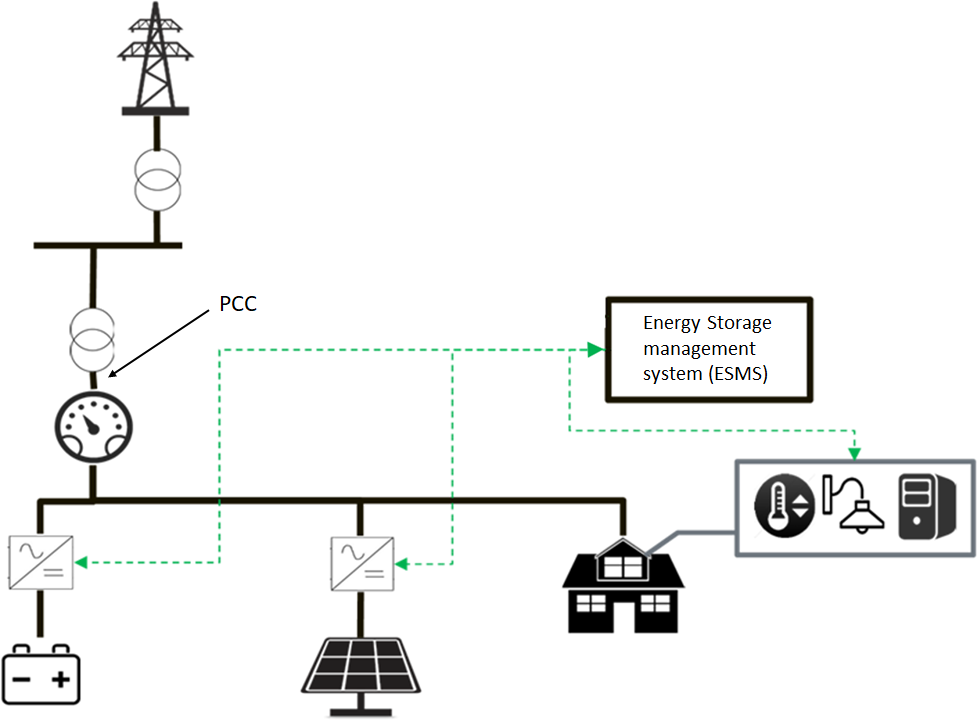
\includegraphics[width=0.45\textwidth]{figs/System_architecture.png}
\caption{Test system architecture}
\label{fig:system_arch}
\vspace{-3mm}
\end{figure}

As seen in the figure the system referenced is a full compared system

For the PV system and the energy storage system, constraints enforced were derived from the physical parameters of the hardware in consideration. The physical bounds (constraints) and price rates associated with the solar power systems are summarized in the Table \ref{tab:solar_pv} and the physical constraints are given by
\vspace{-2mm}
\begin{eqnarray}
\underbar{$Q$}_{_{PV}}\leq Q_{_{PV}}(t_{_k}) \leq \overbar{Q}_{_{PV}}, \\
P^2_{_{PV}}(t_{_k})+Q^2_{_{PV}}(t_{_k})\leq S^2_{_{PV}},
\end{eqnarray}
where
\begin{eqnarray}
\overbar{Q}_{_{PV}}= P_{_{PV}}\tan(\arccos(pf_{_{PV}})),\\
\underbar{$Q$}_{_{PV}}= -P_{_{PV}}\tan(\arccos(pf_{_{PV}})).
\end{eqnarray}


\begin{table}[h]
\caption{Specifications for solar power system used in the study}
\label{tab:solar_pv}
\vspace{-5mm}
\begin{center}
\begin{tabular}{|l|c|}
\hline
PV system parameters & Value \\
\hline
Panels Rating & 875 (kW) \\
\hline
Inverter Rating ($S_{_{PV}}$) & 900 (kVA)\\
\hline
Power Factor ($\rho{f_{_{PV}}}$) Range & 0.8-1.0\\
\hline
Maximum Reactive Power ($\overbar{Q}_{_{PV}}$) & 540 (kVAR)\\
\hline
Minimum Reactive Power ($\underbar{$Q$}_{_{PV}}$) & -540 (kVAR) \\
\hline
LCOE$^*$ ($r_{_{PV}}$) & 2.51 (\textcent/kWh)) \\
\hline
\end{tabular}
\end{center}
$^{*} \text{LCOE: Levelized cost of energy}$
\vspace{-5mm}
\end{table}

The energy storage system constraints and price rates are summarized in Table \ref{tab:energy_storage} and the constraints are given by 
\vspace{-2mm}
\begin{eqnarray}
\overbar{Q}_{_{ES}}= P_{_{ES}}\tan(\arccos(pf_{_{ES}})),\\
\underbar{$Q$}_{_{ES}} = -P_{_{ES}}\tan(\arccos(pf_{_{ES}})),\\
\underbar{$Q$}_{_{ES}}\leq Q_{_{ES}}(t_{_k}), \leq \bar{Q}_{_{ES}},\\
P^2_{_{ES}}(t_{_k})+Q^2_{_{ES}}(t_{_k})\leq S^2_{_{ES}}.
\end{eqnarray}


\begin{table}[h]
\caption{Specifications for energy storage system used in the study}
\vspace{-5mm}
\label{tab:energy_storage}
\begin{center}
\begin{tabular}{|l|c|}
\hline
ESS parameters & Value \\
\hline
Battery Rating & 750 (kW) \\
\hline
Inverter Rating ($S_{_{ES}}$) & 750 (kVA)\\
\hline
Maximum State-of-Charge ($\bar{SOC}_{ES}$) & 2190 (kWh) \\
\hline
Minimum State-of-Charge ($\underbar{SOC}_{_{ES}}$) & 219 (kWh) \\
\hline
Power Factor ($\rho{f_{_{ES}}}$) Range & 0.8-1.0\\
\hline
Maximum Reactive Power ($\overbar{Q}_{_{ES}}$) & 450 (kVAR)\\
\hline
Minimum Reactive Power ($\underbar{$Q$}_{_{ES}}$) & -450 (kVAR) \\
\hline
LCOE$^\star$ ($r_{_{ES}}$) & 12.3 (\textcent/kWh)) \\
\hline
\end{tabular}
\end{center}
$^\star \text{LCOE: Levelized cost of energy}$
%\vspace{-5mm}
\end{table}

To perform the simulations, data related to the distribution network, solar generation profiles, load profiles, and an example feeder were obtained from the available open source databases. The load profile for the distribution network used in this study was obtained from the SUNGRIN project database, which has network model data and load profiles from various feeders located around the state of Florida \cite{sungrin}. Fig. \ref{fig:load_profile} presents an actual load profile with the maximum, minimum, and average power requirement for a 24 h window of a feeder network used in the study. It is important to note that this study used the actual solar irradiance and load profile values obtained from the SUNGRIN project database as the predicted values.  The results will degrade when perfect knowledge does not exist. 

\begin{figure}[!htbp]
\centering
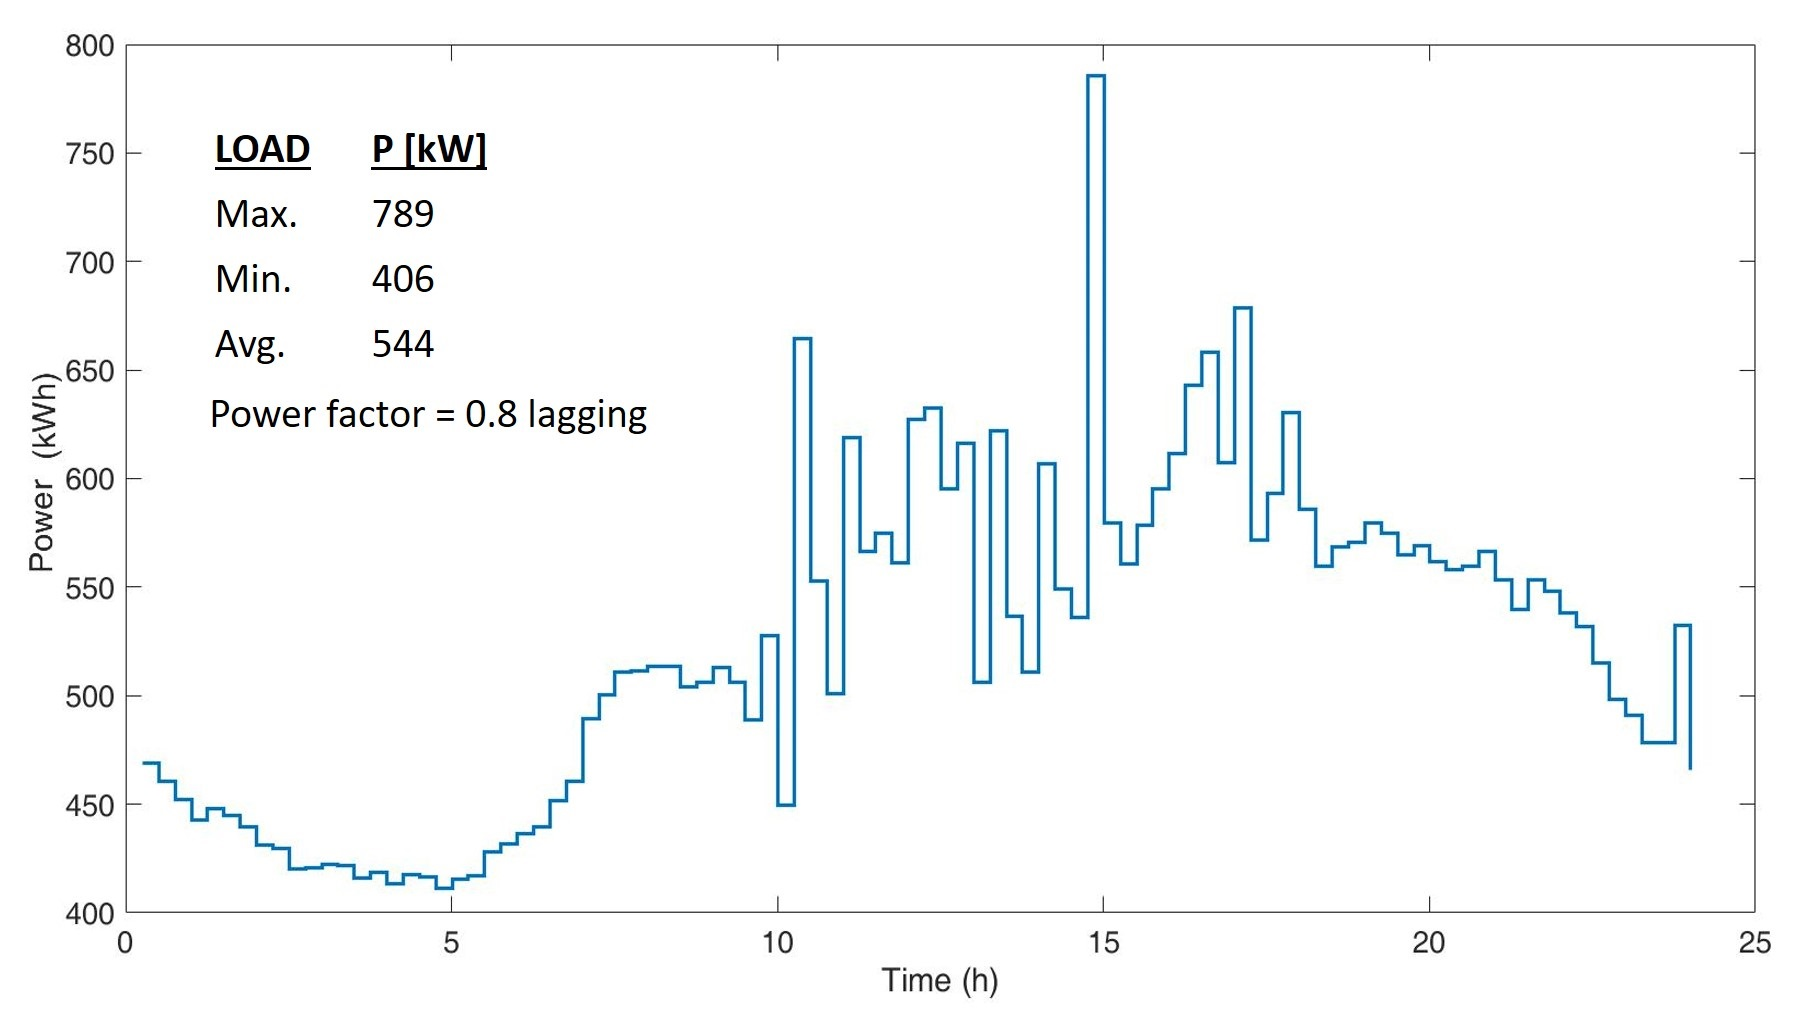
\includegraphics[width=0.45\textwidth]{figs/Load_profile_24hr.jpg}
\caption{Actual load profile with the maximum, minimum, and average power requirement for a 24 h window of a feeder network used in the study.}
\label{fig:load_profile}
\vspace{-3mm}
\end{figure}

As evidenced by the parameters of Tables \ref{tab:solar_pv} and \ref{tab:energy_storage}, the solar power system and ESS were sized for a large-scale (e.g., commercial, industrial or campus scale) micro-grid application. Using the analysis of \cite{res}, $r_{_{ES}}$, the constant levelized cost of energy (LCOE) for the ESS was derived as
\begin{equation}
r_{_{ES}} = \dfrac{ES_{total}}{(Cycles) (ES_{Cap}) (DoD) (\eta_{r})},
\end{equation}
where $ES_{total}$ is the total price of the ESS, $Cycles$ is the total number of cycles under warranty at depth-of-discharge, $ES_{Cap}$ is the total energy capacity of the ESS, $DoD$ is the desired depth-of-discharge of the ESS, and $\eta_{r}$ is the round trip efficiency of the system.


A modified real-time price (RTP) data set was produced using publicly available New York Independent System Operator's (NYISO) wholesale location-based marginal pricing \cite{NYISO2017}. The modification of the price consists of the addition of an RTP supplier charge made by the hypothetical utility company, plus the biasing of an off-peak or on-peak rate determined by using the energy tariff currently available for the TOU program used by the City of Tallahassee. \cite{tallahassee}. The reason for such modification is to preserve the fluctuating nature of the NYISO price data while placing the values in the range of the TOU prices used by the City of Tallahassee, and, therefore more appropriate to North Florida load patterns and markets. The modified RTP values for the 24 h prediction window with a step size of 15 min is shown in Fig. \ref{fig:rtp_24hr}.


\begin{figure}[!htbp]
\vspace{-5mm}
\centering
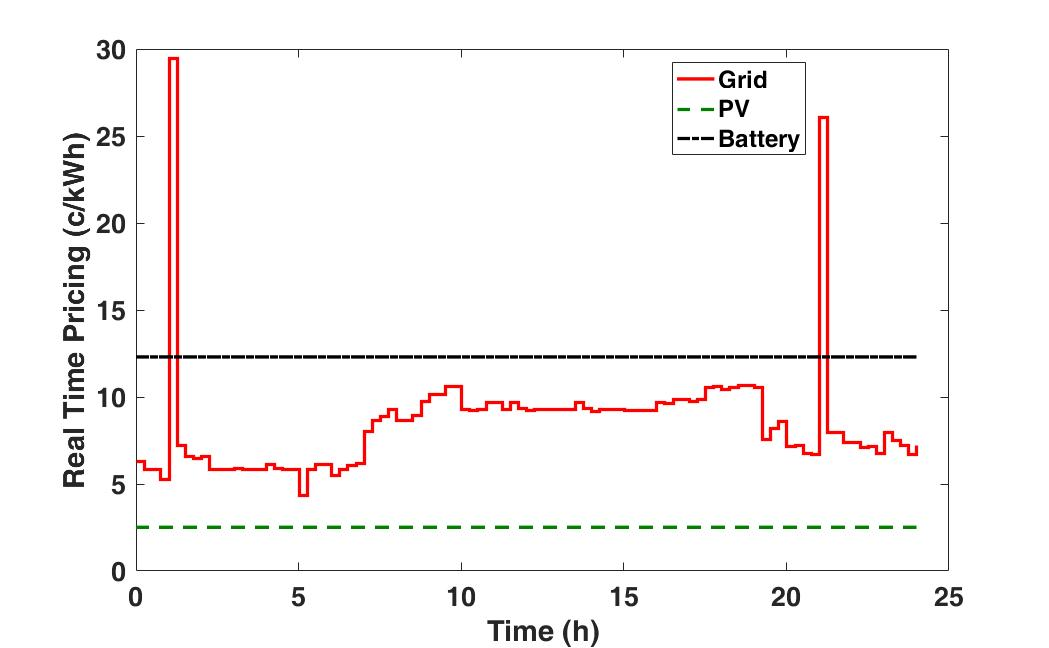
\includegraphics[width=0.5\textwidth]{figs/RTP_24hr_with_der.jpg}
\caption{24 h real-time pricing (RTP) data for grid power for a step size of 15 min used in the study.}
\label{fig:rtp_24hr}
\vspace{-5mm}
\end{figure}



\section{Results and comparison}

( Write about the comparison with real time data from STTR)

\section{Conclusion}

\bibliographystyle{IEEEtran}
\bibliography{mybib.bib}

\ifCLASSOPTIONcaptionsoff
  \newpage
\fi

\end{document}


